\begin{multicols}{2}
\mySection{Maintainance (af dig)}

  \begin{tList}{Hvor kommer gainz fra?}

  \item Spis din mad. Sov din søvn. Spis NOK mad. Sov NOK søvn.
  \item Relativ styrke vs. Absolut styrke - du behøver nok ikke tabe dig.
  \end{tList}

  \begin{tList}{Pas på}
  \item Sener styrkes markant langsommere end muskler.

  \item Hvis du begynder at få ondt i led eller sener, og smerten
    ikke går i sig selv dagen efter, så stop. Du må gerne være lidt
    øm i leddene lige bagefter, men det skal gå i sig selv igen.

  \item Hvis du tropper op til klatring og tænker "wow, jeg kan
    virkelig mærke at jeg hangboardede sidste gang", så skal du gå
    mindre hårdt til den. Der skal ikke bygge sig ømhed op fra uge til uge.
  \end{tList}

  \begin{tList}{Deload}

  \item Hver fjerde uge. Deload betyder bare ingen hang board, ingen pull ups.

  \item Hvorfor?
    Fordi din krop har brug for hvile, også selvom dit sind synes
    du skal give den gas.

  \item Det er tydeligt bevist at deload hjælper kroppen med at
    hvile, og derfor reducerer skadesrisiko. Der er samtidig også en
    chance for at det hjælper dig med at blive stærkere i det lange
    løb, så win-win.

  \item "Jamen jeg trænede faktisk ikke sidste torsdag, så skal jeg
    ikke bare skippe deload den her gang?"
    - Bare følg planen please ...
  \end{tList}

\begin{minipage}{\columnwidth}
\centering
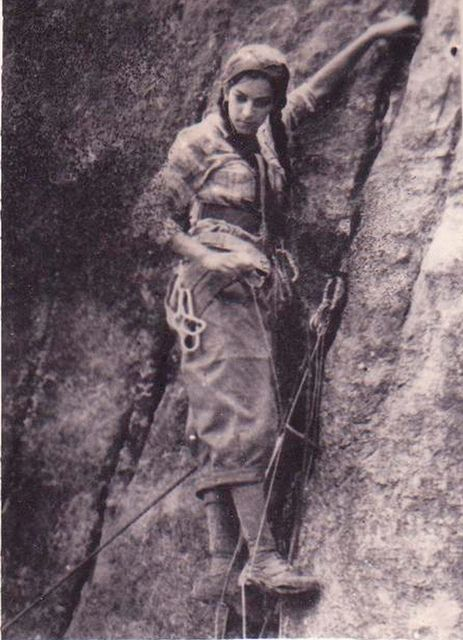
\includegraphics{figs/oldSchoolCool}
\captionof*{figure}{Archana Bhattacharjee (1979)}
\vspace{1em}
\end{minipage}



  \begin{tList}{Du kan hurtigt mærke at du er blevet stærkere?}
  \item   Fedt! Du kan holde
  fast i ting du ikke kunne før, du kan hænge med mere vægt, mindre
  kanter, længere tid osv. Tag den med ro. Det kan være berusende at
  forbedre sig, og det er let at blive grådig. Man får lyst til at
  give den endnu mere gas, og før man har set sig om, har man revet
  et eller andet i stykker. Please don't. Følg planen.
  \end{tList}
\end{multicols}
